\documentclass[crop,tikz]{standalone}

\usepackage{amsmath,marvosym}
\tikzset{>=latex}
\usetikzlibrary{decorations.markings,positioning,arrows}

\begin{document}
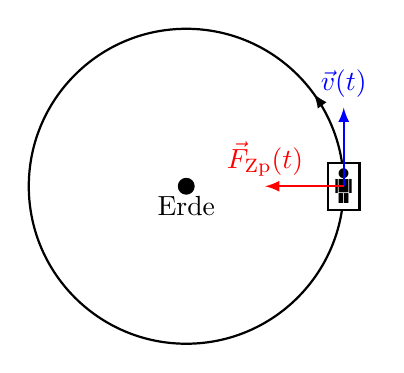
\begin{tikzpicture}[scale=2]
  \draw[fill] (0,0) circle (0.05) node[below] {Erde};
  \draw[thick,
        decoration={markings, mark=at position 0.1 with {\arrow{>}}},
        postaction={decorate}
        ] (0,0) circle (1);
  \pgfmathsetmacro{\cx}{1};
  \pgfmathsetmacro{\cy}{0};
  \pgfmathsetmacro{\cw}{0.2};
  \pgfmathsetmacro{\ch}{0.3};
  \coordinate (P) at (\cx,\cy);
  \draw[fill=white,thick] (\cx-\cw/2,\cy-\ch/2) rectangle (\cx+\cw/2,\cy+\ch/2);
  \node at (P) {\LARGE\Gentsroom};
  \draw[->,blue,thick] (P) -- ++(0,0.5) node[above] {$\vec{v}(t)$};
  \draw[->,red,thick] (P) -- ++(-0.5,0) node[above] {$\vec{F}_\text{Zp}(t)$};
\end{tikzpicture}
\end{document}
